\subsection{A geometric approach}
\label{laserMFnum}

Even though the computation of invariants with the method of
the moving frames is efficient, it is still computationally
prohibitive for very high dimensional flows. For, one has
to compute the invariants with computer algebra, a proccess 
that works\rf{SiminosThesis} for moderate system dimension of the order of $100$,
as required for instance in truncations of \KSe\ studied in \rf{SCD07},
but does not scale well for problems with truncations of order $10,000$ as
a fully resolved $3$-D fluid simulation would easily require\rf{GibsonPhD}.
We will demonstrate in the example of \CLe\ 
how one can use the geometric interpretation of the moving frame method along
with the restriction of the dynamics to a \Poincare\ section
to simply and effectively, yet locally, perform continuous symmetry
reduction in high-dimensional flows.

We have noted that \SOn{2} acts regularly and freely on
$X^*=\Rls{5}\backslash\{x_1=x_2=y_1=y_2=0\}$ and thus we are
guaranteed to find the fundamental invariants by the method
of moving frames if we restrict attention to $X^*$.
Nevertheless the transformations \refeq{eq:invLaser} obtained
by the moving frame method are singular in the subspace
$x_1=x_2=0$.
    \ES{Kevin Mitchell claims that what we do here is
    geometrically impossible because there is a non-removable
    singularity isomorphic to the magnetic monopole string
    singularity. In this section I argue that we do not do it
    globally and this is why it is possible (and we just do
    it!)}
Therefore we would like to ensure that we apply our
reduction procedure only on points away from this subspace. A
way to achieve this is by a judicious choice of \Poincare\
section in original space, \ie~before reduction. Since we are
ultimately interested in reducing the dynamics to a
\Poincare\ return map this suffices for our purposes.
Locating a \Poincare\ section is a non-trivial task
but as we will see in the following, for the procedure to
work we will have to reduce the candidate \Poincare\ sections
to those that are invariant (as a set) under the group
action. 
\ES{dropped: Furthermore we already have gained the insight from
the simpler \Le\ problem that a good choice of section is one
that passes through the \eqva\ that organize the flow. 
}
Here
we are naturally led to choose a section that passes through
the \reqv~\REQV{}{1} such as the section $\mathcal{P}$
defined by $\overline{x}_2-\overline{y}_2=0$ in the variables
of \refeq{eq:invLaser} or by $x_1^2+x_2^2-(x_1 y_1 + x_2
y_2)=0$ in original space and a suitable orientation
condition so that trajectories intersect the section away
from $x_1=x_2=0$ subspace. Here the orientation condition has
be chosen so that trajectories intersect $\mathcal{P}$ moving
from the ``outside'' of the section in
\reffig{fig:CLEmartini} to the ``inside''. Since
$\mathcal{P}$ has been defined by a condition in invariant
variables \refeq{eq:invLaser} it turns out to be
$\SOn{2}$-invariant in the full space. Therefore the group
orbit of any point on $\mathcal{P}$ lies on $\mathcal{P}$. In
\reffig{fig:CLEmartini} the group orbits of the points of
intersection of \rpo~\cycle{01} are visualized as circles
on $\mathcal{P}$.

The next step is to choose a representative out of each group
orbit by means of a slice $\mathcal{K}$ that
intersects each group orbit exactly once. The existence of a
section is guaranteed from \refPro{pro:crossExists}, and the
restriction of the problem to a Poincar\'e section on which the
group \emph{acts} freely. Here we choose $x_1=0$ for
$\mathcal{K}$. Geometrically this is equivalent to rotating
each point of intersection on $\mathcal{K}$ by an appropriate
angle so that it lies on $\mathcal{K}$, exactly as prescribed
by the moving frame \refeq{eq:CLEmf}. This rotation, a linear
operation for any given point, can be applied efficiently
even in high dimensional space when the rotation group
representation is a direct sum of irreducible
representations, as is frequently the case with truncations
of PDEs. Of course, the transformation is still non-linear
through the dependence on the angle and equivalent to the
explicit transformations \refeq{eq:invLaser}.

%%%%%%%%%%%%%%%%%%%%%%%%%%%%%%%%%%%%%%%%%%%%%%%%%%%%%%%%%%%%%%%%%%
\begin{figure}[ht]
\begin{center}
  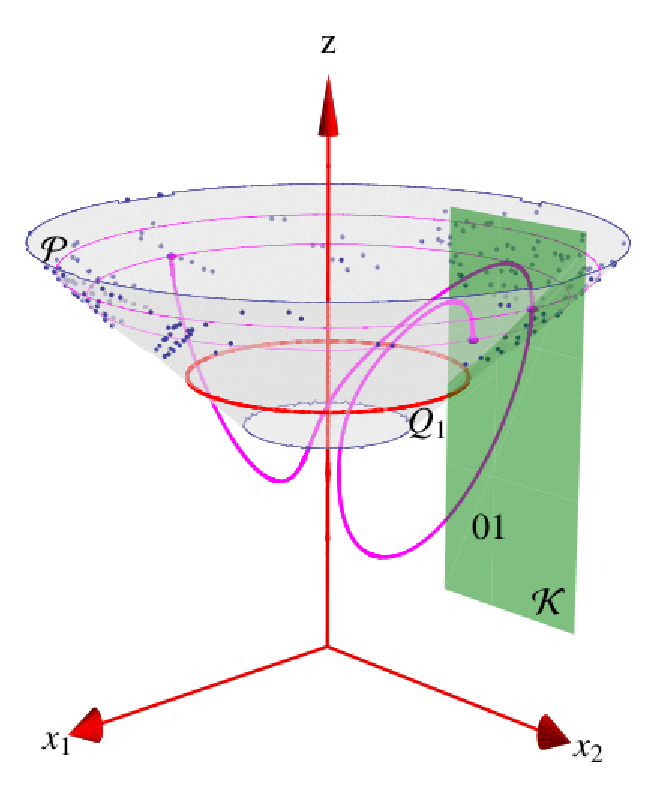
\includegraphics[width=0.35\textwidth]{../figs/CLEmartini}
\end{center}
\caption{
Use of \Poincare\ surface of section $\mathcal{P}$ and
{\csection} $\mathcal{K}$ for symmetry reduction of \CLe\
dynamics with $e=1/10$, $\ImrCLor=0$. Group orbits of the
points of intersection of \rpo\ \cycle{01} are visualized as
circles.
    }
\label{fig:CLEmartini}
\end{figure}
%%%%%%%%%%%%%%%%%%%%%%%%%%%%%%%%%%%%%%%%%%%%%%%%%%%%%%%%%%%%%%%%
